\section{Gramática libre de contexto no ambigua}
	\subsection{Descripción del problema}
	En este problema se debe de construir una única derivación por la izquierda para una cadena de paréntesis balanceada. Usando las siguiente GIC.
	\begin{gather*}
	B \to (RB | \epsilon \\
	R \to ) |  (RR \\
	\end{gather*}
	En donde $B$ es el símbolo inicial y R genera cadenas que tienen un paréntesis derecho más que uno izquierdo.
	\\Si necesitamos expandir B entonces usamos $B \to (RB $ si el siguiente símbolo es $"("$ y $\epsilon$ al final.
	\\Si necesitamos expandir R, usamos $R \to ) $ si el siguiente símbolo es $")"$ y (RR si es $"("$ \cite{WEB}
	El debe contener un modo manual y automático, en el modo manual el usuario ingresara una cadena de paréntesis y sera procesada hasta llegar a una cadena final que nos indicara si la cadena esta balanceada o no.
	\\Por otro lado, en el modo automático se genera una cadena aleatoria de paréntesis con longitud $0 \le n \le 1000 $ que recibirá el mismo tratamiento que en el modo manual.
	\subsection{Código}
	El código fue realizado en Python 3.5.
	\\Archivo: main\_webay.py
	\begin{lstlisting}[language=Python]
	# main_parseo.py
	# -*- coding: utf-8 -*-
	from __future__ import print_function
	from parseo import proceso
	import random

	separador = '='*50
	def iniciar():
	    continuar = True
	    while continuar:
	        opcion = imprimir_menu()
	        if opcion == 1:
	            entrada_consola()
	        elif opcion == 2:
	            ejecutar_random()
	        else:
	            break
	        print('=' * 100)
	        opcion = input("Reintentar [s/n]: ")
	        if opcion.lower() != 's':
	            continuar = False

	    print('Saliendo del programa...')

	def imprimir_menu():
	    print('\n\n%sMenu%s' % (separador, separador))
	    print("""
	        1.- Entrada en consola (Manual)
	        2.- Aleatorio (Automatico)
	        3.- Salir
	    """)
	    try:
	        opcion = int(input("Selecciona una opcion valida: "))
	        return opcion
	    except Exception as e:
	        print('Error ', e)
	        return 0

	def entrada_consola():
	    texto = input("Escribe la cadena de parentesis: ")
	    proceso(texto)

	def ejecutar_random():
	    i = 0
	    longitud_random = random.randint(1, 20)
	    cadena = ''
	    while i < longitud_random:
	        cadena += random.choice(['(', ')'])
	        i += 1

	    print("La cadena es: ", cadena)
	    proceso(cadena)

	iniciar()
	\end{lstlisting}
	Archivo: parseo.py
	\begin{lstlisting}[language=Python]
	# parseo.py
	# -*- coding: utf-8 -*-
	from __future__ import print_function

	def proceso(cadena):
	    derivacion = 'B'
	    archivo = open('historia-parentesis.txt', 'w')
	    cadena += ' '
	    print('Cadena: ', cadena)
	    archivo.write('Cadena: %s'%cadena)
	    continuar = True
	    for simbolo in cadena:
	        if not continuar:
	            break
	        print(derivacion, end = '\t')
	        archivo.write('\n%s   ' %derivacion)
	        for paso in derivacion:
	            if paso == 'B':
	                if simbolo == '(':
	                    derivacion = derivacion.replace('B', '(RB', 1)
	                    print('Regla usada: B->(RB')
	                    archivo.write('Regla usada: B->(RB')
	                    break
	                elif simbolo == ' ':
	                    derivacion = derivacion.replace('B', '', 1)
	                    print('Regla usada: B->e')
	                    archivo.write('Regla usada: B->e')
	                    break
	                elif simbolo == ')':
	                    continuar = False
	                    break
	            elif paso == 'R':
	                if simbolo == ')':
	                    derivacion = derivacion.replace('R', ')', 1)
	                    print('Regla usada: R->)')
	                    archivo.write('Regla usada: R->)')
	                    break
	                elif simbolo == '(':
	                    derivacion = derivacion.replace('R', '(RR', 1)
	                    print('Regla usada: R->(RR')
	                    archivo.write('Regla usada: R->(RR')
	                    break
	                elif simbolo == ' ':
	                    continuar = False
	                    break
	    archivo.write('\nFinal: %s' %derivacion)
	    print('\nFinal: ', derivacion)
			if paso == 'B' and simbolo == ' ':
		        print('\nCadena balanceada')
		        archivo.write('\nCadena balanceada')
		    else:
		        print('\nCandena no balanceada')
		        archivo.write('\nCadena no balanceada')
	    archivo.close()
	\end{lstlisting}
	\subsection{Pruebas}
	Pruebas de las opciones del menú.
	\\
	{\large Modo de consola.}
	\begin{figure}[H]
		\begin{center}
			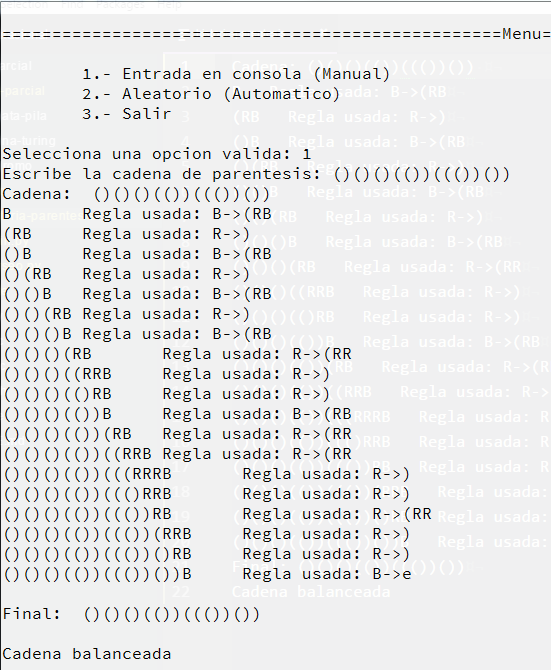
\includegraphics[width=11cm, height=10cm]{img/parseo-manual-consola.png}
			\caption{Historia de las derivaciones en consola.}
			\label{fig:parseo1}
		\end{center}
	\end{figure}
	\begin{figure}[H]
		\begin{center}
			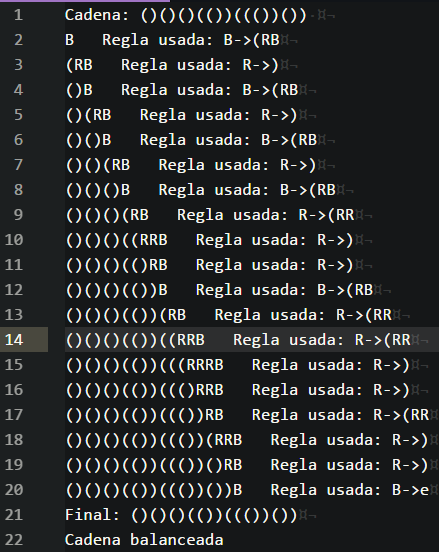
\includegraphics[width=9cm, height=7cm]{img/parseo-manual-archivo.png}
			\caption{Parte de la historia de las derivaciones en archivo.}
			\label{fig:parseo2}
		\end{center}
	\end{figure}
	{\large Modo automático}
	\begin{figure}[H]
		\begin{center}
			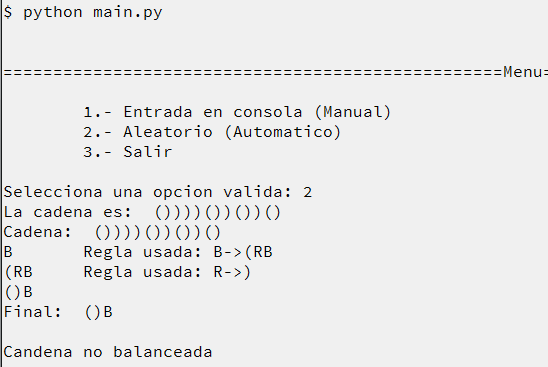
\includegraphics[width=\linewidth, height=9cm]{img/parseo-automatico-consola.png}
			\caption{Modo automático desde consola.}
			\label{fig:parseo3}
		\end{center}
	\end{figure}
	\begin{figure}[H]
		\begin{center}
			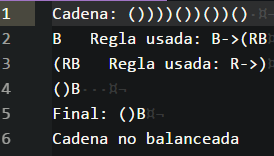
\includegraphics[width=12cm, height=7cm]{img/parseo-automatico-archivo.png}
			\caption{Historia del modo automático en archivo.}
			\label{fig:parseo4}
		\end{center}
	\end{figure}
